\section{Shutdown}

\begin{figure}[h!]
  \begin{sequencediagram}
    \newinst{wallet}{\shortstack{Customer wallet \\
      \\ 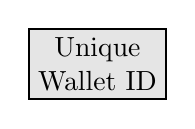
\begin{tikzpicture}
        \node [fill=gray!20,draw=black,thick,align=center] { Unique \\ Wallet ID};
      \end{tikzpicture}
    }}
    \newinst[2]{exchange}{\shortstack{Taler (exchange) \\
       \\ \begin{tikzpicture}[shape aspect=.5]
        \tikzset{every node/.style={cylinder,shape border rotate=90, draw,fill=gray!25}}
        \node at (1.5,0) {\shortstack{{{\tiny Database}}}};
       \end{tikzpicture}
    }}
    \newinst[2]{bank}{\shortstack{Customer bank \\
      \\ 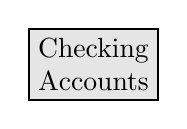
\begin{tikzpicture}
        \node [fill=gray!20,draw=black,thick,align=center] {Checking \\ Accounts};
      \end{tikzpicture}
    }}
    \postlevel

    \begin{callself}{exchange}{Operator initiates shutdown}{}
    \end{callself}
     \mess[0]{exchange}{{Shutdown alert}}{wallet}
     \begin{sdblock}{Bank account known?}{}
       \begin{callself}{wallet}{Designate bank account}{}
       \end{callself}
     \end{sdblock}
    \mess[0]{wallet}{{Deposit (Coins)}}{exchange}
    \begin{sdblock}{Acceptable account?}{}
    \mess[0]{exchange}{{Refuse deposit}}{wallet}
    \end{sdblock}
    \begin{sdblock}{KYC/AML required?}{}
    \begin{callself}{exchange}{Figures~\ref{fig:proc:kyc}, \ref{fig:proc:aml}}{}
    \end{callself}
    \end{sdblock}
    \mess[0]{exchange}{{Initiate transfer}}{bank}
\end{sequencediagram}
  \caption{Shutdown interactions between customer, Taler exchange (payment
    service provider) and bank.}
  \label{fig:int:shutdown}
\end{figure}

KYC/AML requirements are relaxed in cases where the customer is able to
cryptographically demonstrate that they previously withdrew these coins from
the designated checking account.  Thus, KYC/AML checks here primarily still
apply if the customer received the funds via P2P transfers from other wallets.
